\chapter{要素技術}
\label{chap:elemental}
本章では,本研究に関連する要素技術を述べる
\section{深層学習}
\subsection{教師あり学習}
教師あり学習は,機械学習の一種であり,
データセットと呼ばれる
ラベル付きのデータの集合を使用してモデルを訓練する手法である.
データセットには,入力データとそれに対応する正解(ラベル)が含まれている.
モデルはデータセットを利用して,正解となる出力を得られるように学習を行っていく.

\subsection{end-to-end学習}
\ref{fig:e2e}に示すように,入力されるデータから目的の出力を得るために必要なデータを得るために必要な
他段階の処理をニューラルネットワークを用いて直接学習する手法である.
自律移動を例に述べる.
人物や障害物などの物体認識,走行レーンの検出,
経路計画,ステアリング制御などの複数個のタスクを解く必要があるが, 
end-to-end学習では先程のタスクを人間が直接設定せずに
カメラ画像をニューラルネットワークに入力することで,
直接ステアリング操作を学習する.
\begin{figure}[htbp]
    \centering
     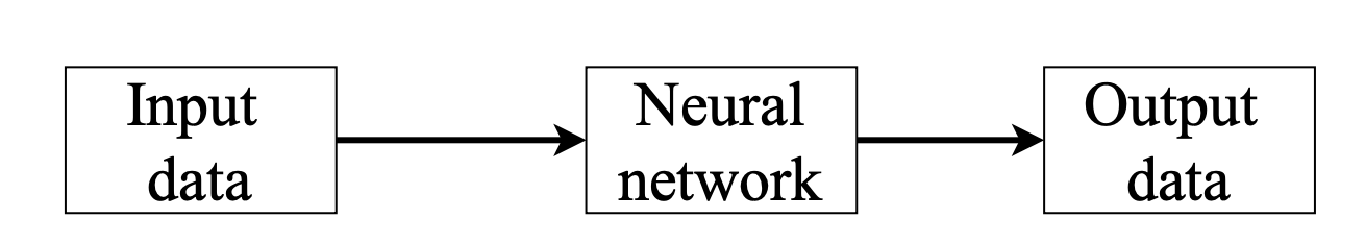
\includegraphics[width=90mm]{images/pdf/e2e.pdf}
     \caption{Structure of end-to-end learning}
     \label{fig:e2e}
\end{figure}

\newpage
\section{メトリックマップに基づくナビゲーション}
一般的に,移動ロボットを目的地まで誘導する制御はナビゲーションと呼ばれている.
その中で,事前にLiDARやオドメトリなどのセンサを使用して作成した占有格子地図などの
地図を用いたナビゲーション手法がある.
本稿ではこの地図に基づくナビゲーションを
「メトリックマップに基づくナビゲーション」と呼ぶ.
このメトリックマップに基づくナビゲーションを提供するルールベース制御器として
ROS Navigation stack\cite{ros}がある.
\begin{quote}
    \begin{itemize}
     \item パーティクルフィルタによって自己位置推定を行うモンテカルロ自己位置推定(MCL)
     \item 障害物認識などの局所的または地図全体の大域的なコスト計算と,その結果に基づく経路計画
     \item 経路に追従する並進速度や角速度などの速度指令
    \end{itemize}
   \end{quote}
この中で,経路を追従する行動を「経路追従行動」と呼ぶ.
本論文では,Navigation stackをこの模倣学習やデータセットの作成に使用している.
% \vspace{5zh}
\begin{figure}[htbp]
    \centering
     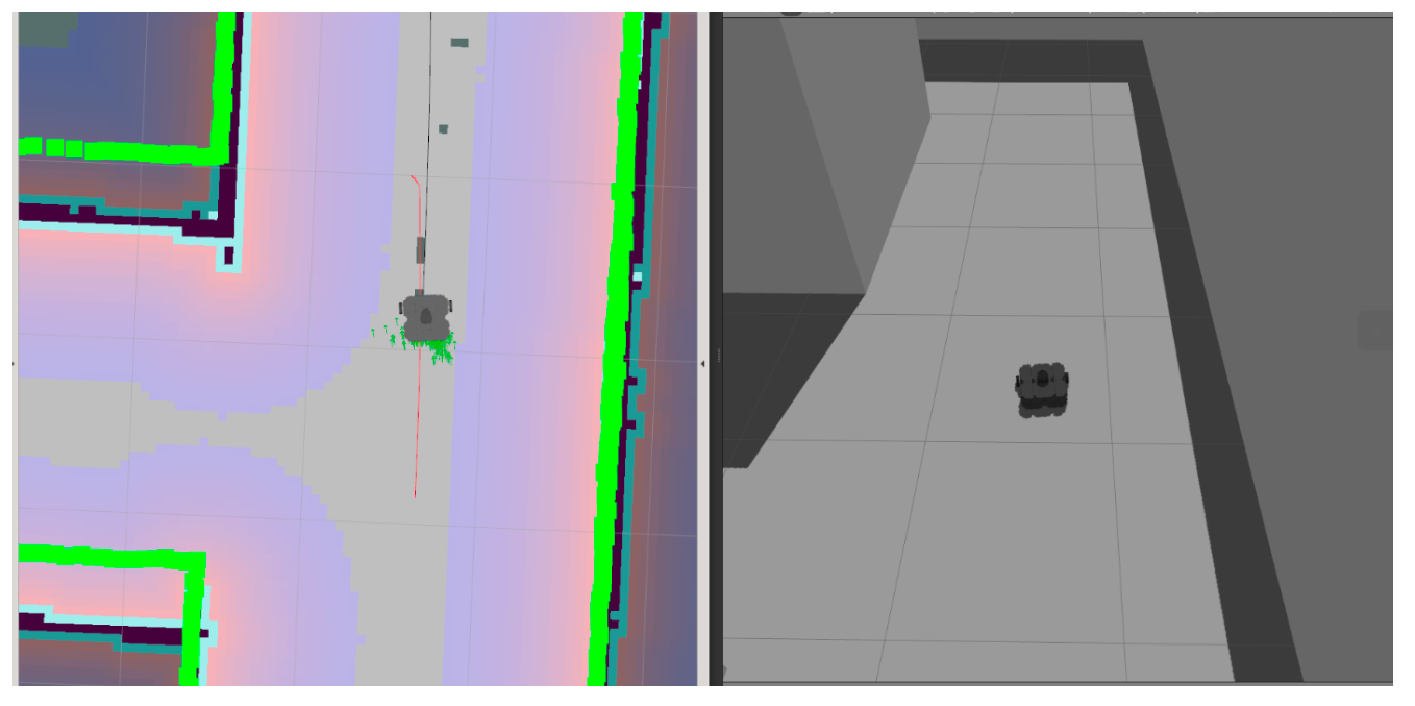
\includegraphics[width=100mm]{images/pdf/nav.pdf}
     \caption{Path-following module system Quoted from\cite{shimada2020}}
     \label{fig:nav}
\end{figure}

\newpage
\section{トポロジカルマップ}
トポロジカルマップは,環境中のランドマークなどの
特徴的な箇所(ノード)とその繋がり(エッジ)によって
環境を表現したマップである.
島田らは\ref{fig:topo}に示すようなトポロジカルマップの形式\cite{shimada2020}を提案している
トポロジカルマップのノードは,
人の道案内に関するアンケートにおいて,
通路の特徴が多用されていたため,該当する位置に配置され,
その位置がどのような通路の特徴であるかという情報を
持っている.また,「直進」や「右折」といった~で述べるシナリオの行動から
移動するエッジを選択するために,ノードはエッジのIDと相対角度の情報を
持っている.エッジはノードの接続関係を表すように
ノード同士を結んでいる.多くの研究では距離に関する情報を持っていることが
多いが,島田らの形式ではIDのみを持っている.
本稿で用いるトポロジカルマップは,島田らが提案した形式を指す.
\begin{figure}[htbp]
    \centering
     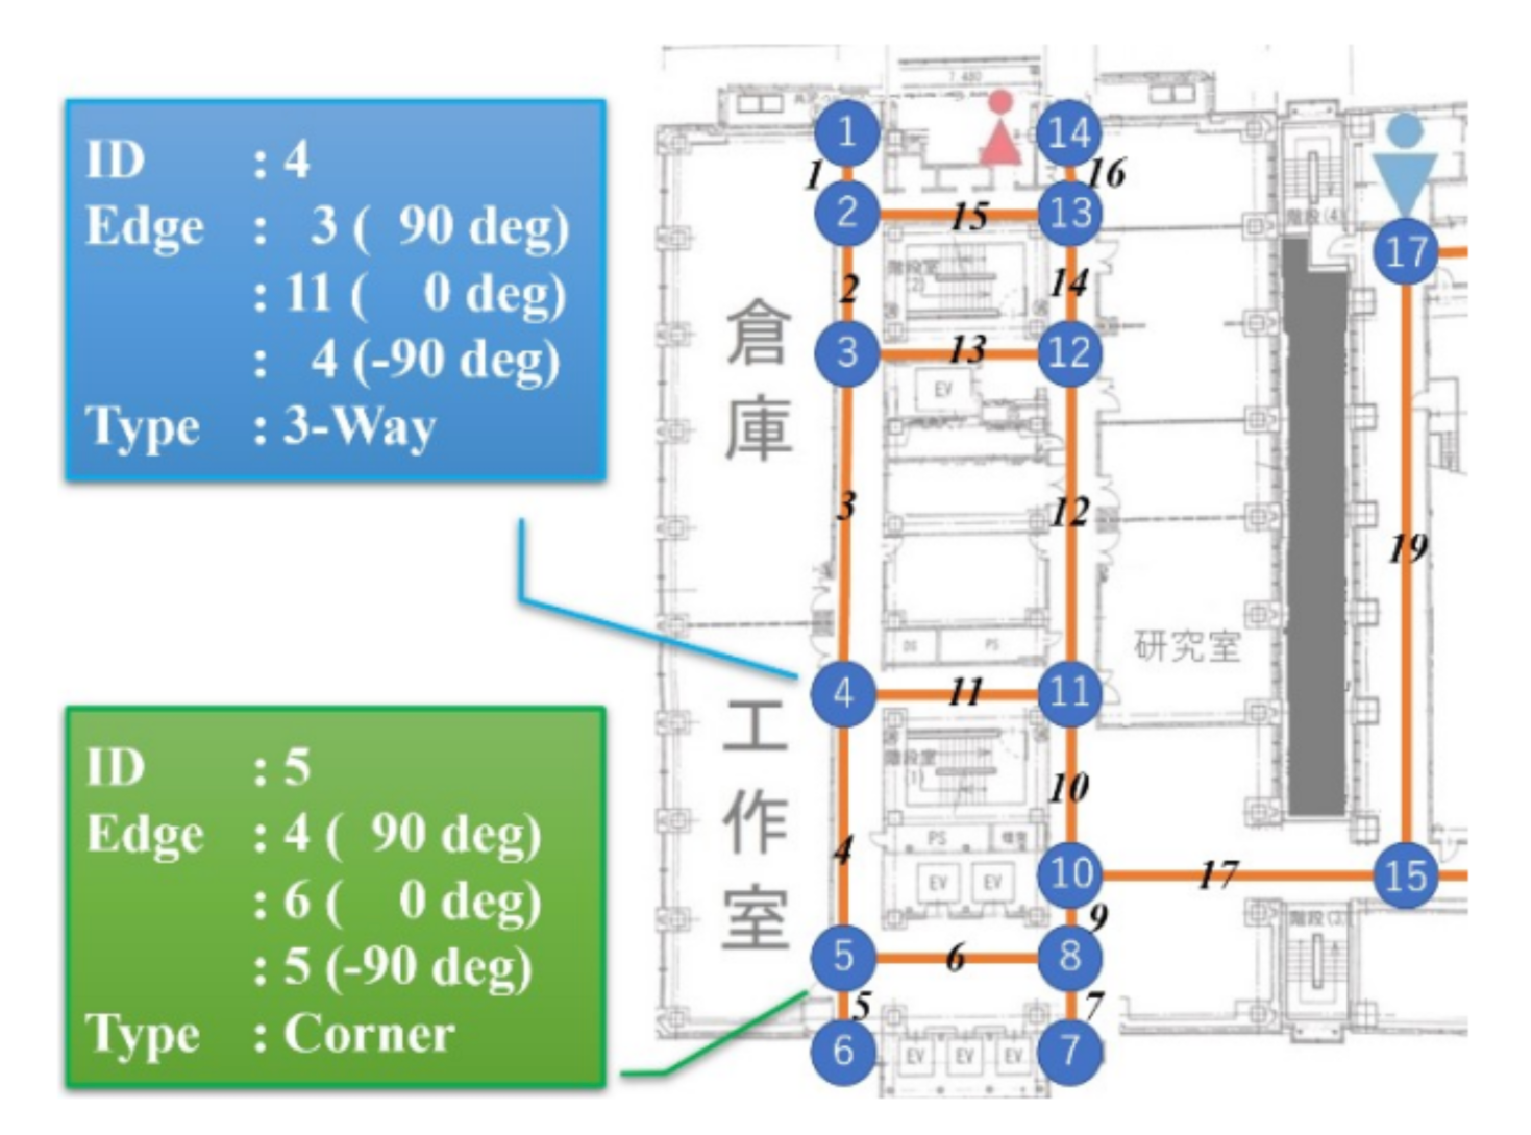
\includegraphics[width=90mm]{images/pdf/topo.pdf}
     \caption{Path-following module system Quoted from\cite{shimada2020}}
     \label{fig:topo}
\end{figure}
\newpage
\section{シナリオ}
シナリオはトポロジカルマップ上での,目的地までの経路を単語の組み合わせで表現したものである,
シナリオは「次の角」や「突き当たり」のような「条件」と「直進」,「右折」のような「行動」の組み合わせにより作成される.
このシナリオの形式は,トポロジカルマップと同様に
人の道案内に関するアンケートで得た,
「次の角まで」のような「条件」と「左折」などの「行動」を組み合わせているという
情報を基に決定している,
例えば,\ref{fig:scenario01}に示すような経路をシナリオで表すと,「3番目の三叉路まで直進.停止」となる,
\begin{figure}[htbp]
    \centering
     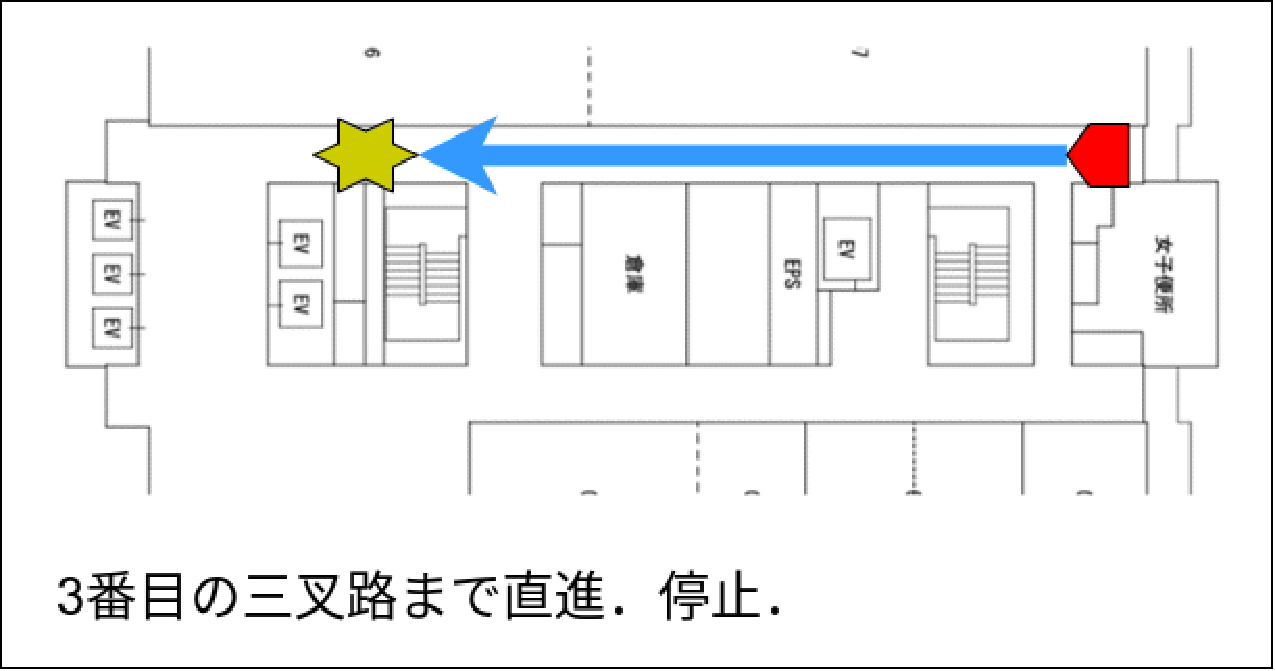
\includegraphics[width=90mm]{images/pdf/scenario/scenario01.pdf}
     \caption{Path-following module system Quoted from\cite{shimada2020}}
     \label{fig:scenario01}
\end{figure}